\documentclass[
    %twoside,
]{ctexbook}
\usepackage[
% paperheight=16cm, 
% paperwidth=12cm,% Set the height and width of the paper
includehead,
% nomarginpar,% We don't want any margin paragraphs
% % textwidth=10cm,% Set \textwidth to 10cm
headheight=14pt,% Set \headheight to 10mm
]{geometry}
% \usepackage{ctex}
\usepackage{xcolor}

\usepackage{tikz}
\usepackage{graphicx}% Include figure files
\usepackage{braket}% Dirac notations
\usepackage{enumitem}
\usepackage{fancyhdr}
\usepackage{fontspec}
\usepackage{titlesec}
\usepackage{titletoc}  
\usepackage{fourier-orns} % 
\usepackage{hyperref}   % bookmarks
\usepackage{url}        % hyperlinks
\usepackage{amssymb,amsmath,mathtools}
\usepackage{amsthm}

\usepackage{framed}
\usepackage{tcolorbox}

\usepackage{wrapfig} %Wrapping text around figures

\usepackage{import}
\usepackage{natbib}
\usepackage{txfonts} % for \ointctrclockwise
\usepackage{appendix} %加入附录需使用appendix宏包
\raggedbottom



\usetikzlibrary{quotes,angles}
\usetikzlibrary {arrows.meta}
\usetikzlibrary{decorations.markings}

\hypersetup{
    colorlinks=true,
    linkcolor=blue,
    filecolor=magenta,      
    urlcolor=cyan,
    pdftitle={},
    pdfpagemode=FullScreen,
    }

% \usepackage{zhnumber}

\usepackage{titling} % to customize \maketitle
\usepackage{cases} 

\renewcommand{\headrule}{%
\vspace{-8pt}\hrulefill
\raisebox{-2.1pt}{\quad\decofourleft\decotwo\decofourright\quad}\hrulefill}


\newtcolorbox{examplebox}[1]{
  colbacktitle=yellow!50!white,
  coltitle=black,
  colback=white,
  colframe=yellow!75!black,
  fonttitle=\bfseries,
  title={例:#1}
}
% \newtheorem{Definition}{\hspace{2em}定义}[subsection]
% \newtheorem{Definition}{\hspace{2em}定义}[section]
% \newtheorem{Definition}{\hspace{2em}定义}[chapter]
\newtheorem{Definition}{\hspace{2em}定义}[]
\renewcommand{\proofname}{\indent\bf 证明:}
\renewcommand{\qedsymbol}{$\blacksquare$}    % 证毕符号改成黑色的正方形

\newenvironment{solution}{\begin{proof}[\indent\bf 解]}{\end{proof}}


\newcommand{\solutionbox}[1]{
  \begin{framed}
    \setlength{\fboxrule}{2pt}
    \setlength{\fboxsep}{10pt}
    \setlength{\FrameSep}{20pt}
    % \setlength{\cornersize}{0.3cm}
    \noindent\textbf{解}: #1
  \end{framed}
}



\begin{document}

\pagestyle{fancy}

% \renewcommand{\chaptermark}[1]{\markboth{\CTEXthechapter\quad #1}{}}
% \renewcommand{\sectionmark}[1]{\markright{\CTEXthesection\quad #1}}
% \renewcommand{\sectionmark}[1]{\markleft{\CTEXthesection\quad #1}}

% \fancyhf{}
% \fancyhead[LE]{\nouppercase{\rightmark\hfill\leftmark}}
% \fancyhead[RO]{\nouppercase{\leftmark\hfill\rightmark}}

%... then configure it.
\fancyhead{} % clear all header fields
% \fancyhead[LE]{\textbf{PHYS}}
% \fancyhead[L]{\textbf{\leftmark}}
% \fancyhead[L]{\chaptermark{}}
% \fancyhead[L]{\sectionmark{}}
\fancyhead[LE]{\textbf{\leftmark}}
\fancyhead[RO]{\textbf{\rightmark}}

% \fancyhead[LO]{\textbf{Kai Luo}}
% \fancyhead[LO]{罗凯}

% \fancyhead[LE]{\nouppercase{\rightmark\hfill\leftmark}}
% \fancyhead[RO]{\nouppercase{\leftmark\hfill\rightmark}}

\fancyfoot{} % clear all footer fields
% \fancyfoot[CE,CO]{\rightmark}
% \fancyfoot[LO,CE]{}
% \fancyfoot[CO,RE]{Nanjing University of Science and Technology}
\fancyfoot[C]{\thepage}
% \fancyfoot[CE,O]{\thechapter}

% \ctexset{
%     part={
%         % format+ = \zihao{-2} \heiti \raggedright,
%         % format+ = \zihao{-1} \heiti,
%         % format+ =  \heiti  \centering,
%         name = {},
%         number = 第\chinese{part}篇,
%         % beforeskip = 1.0ex plus 0.2ex minus .2ex,
%         % afterskip = 1.0ex plus 0.2ex minus .2ex,
%         % aftername = \hspace{15pt}
%     },
%     chapter={
%         % format+ = \zihao{-2} \heiti \raggedright,
%         % format+ = \zihao{-2} \heiti,
%         name = {},
%         number = 第\chinese{chapter}章,
% 		% beforeskip = 1.0ex plus 0.2ex minus .2ex,
% 		% afterskip = 1.0ex plus 0.2ex minus .2ex,
% 		% aftername = \hspace{10pt}
%     },
% 	section={
% 		%format用于设置章节标题全局格式,作用域为标题和编号
% 		%字号为小三,字体为黑体,左对齐
% 		%+号表示在原有格式下附加格式命令
% 		% format+ = \zihao{-3} \heiti, %\raggedright,
% 		%name用于设置章节编号前后的词语
% 		%前、后词语用英文状态下,分开
% 		%如果没有前或后词语可以不填
% 		% name = {},
% 		%number用于设置章节编号数字输出格式
% 		%输出section编号为中文
% 		number = 第\chinese{section}节
% 		% %beforeskip用于设置章节标题前的垂直间距
% 		% %ex为当前字号下字母x的高度
% 		% %基础高度为1.0ex,可以伸展到1.2ex,也可以收缩到0.8ex
% 		% beforeskip = 1.0ex plus 0.2ex minus .2ex,
% 		% %afterskip用于设置章节标题后的垂直间距
% 		% afterskip = 1.0ex plus 0.2ex minus .2ex,
% 		% %aftername用于控制编号和标题之间的格式
% 		% %\hspace用于增加水平间距
% 		% aftername = \hspace{10pt}
% 	},
% 	subsection={
% 		% format + = \centering,
% 		% format+ = \zihao{5} \kaishu \raggedright,
% 		% format+ = \zihao{4}, %\raggedright,
% 		%仅输出subsection编号且为中文
% 		% number = \arabic{subsection}, %\chinese{subsection},
%         number = 第\arabic{section}.\arabic{subsection}讲,
% 		% name = {,.},
% 		% beforeskip = 1.0ex plus 0.2ex minus .2ex,
% 		% afterskip = 1.0ex plus 0.2ex minus .2ex,
% 		% aftername = \hspace{3pt}
% 	},
% 	subsubsection={
% 		%设置对齐方式为居中对齐
% 		% format+ = \zihao{5} \fangsong \centering,
% 		% format + = \centering,
% 		%仅输出subsubsection编号,格式为阿拉伯数字,打字机字体
% 		% number = \ttfamily\arabic{subsubsection},
%         % number = 第\arabic{section}.\arabic{subsection}.\arabic{subsubsection}点,
%         number = 第\arabic{section}.\arabic{subsection}.\arabic{subsubsection}条,
% 		% name = {},
% 		% beforeskip = 1.0ex plus 0.2ex minus .2ex,
% 		% afterskip = 1.0ex plus 0.2ex minus .2ex,
% 		% aftername = \hspace{0pt}
% 	}
% }



\newcommand{\sssub}[1]{ {\mathrm{#1} }}  % script size subscript\\\
\newcommand{\funcd}[2]{ \frac{d{#1}}{d{#2}}} %function full derivative
\newcommand{\funcpd}[2]{ \frac{\partial{#1}}{\partial{#2}}} %function partial derivative
\newcommand{\fnald}[2] { \frac{\delta {#1}}{\delta {#2}}} % functional derivative

\def\ext{\sssub{ext}}
\def\x{\sssub{x}}
\def\xc{\sssub{xc}}
\def\H{\sssub{H}}
\def\Hx{\sssub{Hx}}
\def\Hxc{\sssub{Hxc}}
\def\c{\sssub{c}}
\def\s{\sssub{s}}

% \def\ext{\sssub{ext}}
% \def\ext{\sssub{ext}}
% \def\ext{\sssub{ext}}
% \def\ext{\sssub{ext}}
% \defsssub{ext}


% definitions of bold faced symbols
\def\brpppp{{\mathbf{r}^{\prime\prime\prime\prime}}}
\def\brppp{{\mathbf{r}^{\prime\prime\prime}}}
\def\brpp{{\mathbf{r}^{\prime\prime}}}
\def\brp{{\mathbf{r}^{\prime}}}
\def\bzp{{\mathbf{z}^{\prime}}}
\def\bxp{{\mathbf{x}^{\prime}}}
\def\tp{{{t}^{\prime}}}
\def\tpp{{{t}^{\prime\prime}}}
\def\tppp{{{t}^{\prime\prime\prime}}}

\def\tbr{{\tilde{\mathbf{r}}}}
\def\bk{{\mathbf{k}}}
\def\br{{\mathbf{r}}}
\def\bp{{\mathbf{p}}}
\def\bq{{\mathbf{q}}}
\def\bv{{\mathbf{v}}}
\def\bz{{\mathbf{z}}}
\def\mbf{{\mathbf{f}}}

\def\bx{{\mathbf{x}}}
\def\bR{{\mathbf{R}}}
\def\bM{{\mathbf{M}}}
\def\bP{{\mathbf{P}}}
\def\bT{{\mathbf{T}}}
\def\bK{{\mathbf{K}}}
\def\bA{{\mathbf{A}}}
\def\bB{{\mathbf{B}}}
\def\bD{{\mathbf{D}}}
\def\bE{{\mathbf{E}}}
\def\bF{{\mathbf{F}}}
\def\bG{{\mathbf{G}}}
\def\bH{{\mathbf{H}}}
\def\bI{{\mathbf{I}}}
\def\bJ{{\mathbf{J}}}
\def\bP{{\mathbf{P}}}
\def\bS{{\mathbf{S}}}
\def\bV{{\mathbf{V}}}
\def\bX{{\mathbf{X}}}
\def\bY{{\mathbf{Y}}}
\def\dd{{\mathop{}\!\mathrm{d}}}
\def\dr{{\!\!\dd\br\,}}
\def\dx{{\!\!\dd\bx\,}}
\def\dy{{\!\!\dd\by\,}}
\def\dk{{\!\!\dd\bk\,}}
\def\dG{{\!\!\dd\bG\,}}


\def\half{{\frac{1}{2}}}
\def\tr{{\mathrm{tr}}}


\def\Arg{{\mathrm{Arg}\;}}
\def\arg{{\mathrm{arg}\;}}
\def\Res{{\mathrm{Res}\;}}

% \maketitle

% \begin{figure}
%     \begin{center}
%     \includegraphics[scale=1.5]{tikz/cover_rich.pdf}
%     % \caption{}
%     \end{center}
% \end{figure}
\title{\zihao{1}\heiti 数学物理方法讲义}
\author{\zihao{3}\kaishu 罗凯\\
% \institute[*]{南京理工大学理学院}
% % \institute[*]{School of Science,\\
% % Nanjing University of Science and Technology,\\
% % kluo@njust.edu.cn}
% 南京理工大学理学院, \\
kluo@njust.edu.cn}
% % \email{kluo@njust.edu.cn}
% \date{\zhdigits{2023}年秋}
\date{\fangsong \zhdigits{2023},\zhganzhinian{2023}年秋}

% \begin{titlepage}
\maketitle


% \begin{figure}[!htp]
%     \begin{center}
% \begin{tikzpicture}[scale=1]
  
%     % Draw the background
%     \fill[gray!20] (-3,-3) rectangle (3,3);
    
%     % Draw the contour
%     \draw[black,thick,->] (-2.5,0) -- (2.5,0) node[right] {$\Re(z)$};
%     \draw[black,thick,->] (0,-2.5) -- (0,2.5) node[above] {$\Im(z)$};
    
%     \draw[red, thick] (0.5,0) arc (0:180:0.5);
%     \draw[red, thick] (-0.5,0) -- (-2,0) arc (180:360:2) -- (0.5,0);
    
%     % Draw the labels
%     \draw (-0.5,-0.1) node[below] {$-R$};
%     \draw (0.5,-0.1) node[below] {$R$};
%     \draw (-0.5,2.2) node {$\Gamma_R$};
    
%     % Draw the title
%     % \node[align=center] at (0,0.8) {\Huge };
    
%     % Draw the author
%     % \node[align=center] at (0,-1.2) {\Large by John\\Doe};
    
%   \end{tikzpicture}
% \end{center}
% \end{figure}

% \end{titlepage}

% % \maketitle

% \begin{figure}
%     \begin{center}
%     \includegraphics[scale=1.5]{tikz/cover_rich.pdf}
%     % \caption{}
%     \end{center}
% \end{figure}
\title{\zihao{1}\heiti 数学物理方法讲义}
\author{\zihao{3}\kaishu 罗凯\\
% \institute[*]{南京理工大学理学院}
% % \institute[*]{School of Science,\\
% % Nanjing University of Science and Technology,\\
% % kluo@njust.edu.cn}
% 南京理工大学理学院, \\
kluo@njust.edu.cn}
% % \email{kluo@njust.edu.cn}
% \date{\zhdigits{2023}年秋}
\date{\fangsong \zhdigits{2023},\zhganzhinian{2023}年秋}

% \begin{titlepage}
\maketitle


% \begin{figure}[!htp]
%     \begin{center}
% \begin{tikzpicture}[scale=1]
  
%     % Draw the background
%     \fill[gray!20] (-3,-3) rectangle (3,3);
    
%     % Draw the contour
%     \draw[black,thick,->] (-2.5,0) -- (2.5,0) node[right] {$\Re(z)$};
%     \draw[black,thick,->] (0,-2.5) -- (0,2.5) node[above] {$\Im(z)$};
    
%     \draw[red, thick] (0.5,0) arc (0:180:0.5);
%     \draw[red, thick] (-0.5,0) -- (-2,0) arc (180:360:2) -- (0.5,0);
    
%     % Draw the labels
%     \draw (-0.5,-0.1) node[below] {$-R$};
%     \draw (0.5,-0.1) node[below] {$R$};
%     \draw (-0.5,2.2) node {$\Gamma_R$};
    
%     % Draw the title
%     % \node[align=center] at (0,0.8) {\Huge };
    
%     % Draw the author
%     % \node[align=center] at (0,-1.2) {\Large by John\\Doe};
    
%   \end{tikzpicture}
% \end{center}
% \end{figure}

% \end{titlepage}

% \newcommand{\sssub}[1]{ {\mathrm{#1} }}  % script size subscript\\\
\newcommand{\funcd}[2]{ \frac{d{#1}}{d{#2}}} %function full derivative
\newcommand{\funcpd}[2]{ \frac{\partial{#1}}{\partial{#2}}} %function partial derivative
\newcommand{\fnald}[2] { \frac{\delta {#1}}{\delta {#2}}} % functional derivative

\def\ext{\sssub{ext}}
\def\x{\sssub{x}}
\def\xc{\sssub{xc}}
\def\H{\sssub{H}}
\def\Hx{\sssub{Hx}}
\def\Hxc{\sssub{Hxc}}
\def\c{\sssub{c}}
\def\s{\sssub{s}}

% \def\ext{\sssub{ext}}
% \def\ext{\sssub{ext}}
% \def\ext{\sssub{ext}}
% \def\ext{\sssub{ext}}
% \defsssub{ext}


% definitions of bold faced symbols
\def\brpppp{{\mathbf{r}^{\prime\prime\prime\prime}}}
\def\brppp{{\mathbf{r}^{\prime\prime\prime}}}
\def\brpp{{\mathbf{r}^{\prime\prime}}}
\def\brp{{\mathbf{r}^{\prime}}}
\def\bzp{{\mathbf{z}^{\prime}}}
\def\bxp{{\mathbf{x}^{\prime}}}
\def\tp{{{t}^{\prime}}}
\def\tpp{{{t}^{\prime\prime}}}
\def\tppp{{{t}^{\prime\prime\prime}}}

\def\tbr{{\tilde{\mathbf{r}}}}
\def\bk{{\mathbf{k}}}
\def\br{{\mathbf{r}}}
\def\bp{{\mathbf{p}}}
\def\bq{{\mathbf{q}}}
\def\bv{{\mathbf{v}}}
\def\bz{{\mathbf{z}}}
\def\mbf{{\mathbf{f}}}

\def\bx{{\mathbf{x}}}
\def\bR{{\mathbf{R}}}
\def\bM{{\mathbf{M}}}
\def\bP{{\mathbf{P}}}
\def\bT{{\mathbf{T}}}
\def\bK{{\mathbf{K}}}
\def\bA{{\mathbf{A}}}
\def\bB{{\mathbf{B}}}
\def\bD{{\mathbf{D}}}
\def\bE{{\mathbf{E}}}
\def\bF{{\mathbf{F}}}
\def\bG{{\mathbf{G}}}
\def\bH{{\mathbf{H}}}
\def\bI{{\mathbf{I}}}
\def\bJ{{\mathbf{J}}}
\def\bP{{\mathbf{P}}}
\def\bS{{\mathbf{S}}}
\def\bV{{\mathbf{V}}}
\def\bX{{\mathbf{X}}}
\def\bY{{\mathbf{Y}}}
\def\dd{{\mathop{}\!\mathrm{d}}}
\def\dr{{\!\!\dd\br\,}}
\def\dx{{\!\!\dd\bx\,}}
\def\dy{{\!\!\dd\by\,}}
\def\dk{{\!\!\dd\bk\,}}
\def\dG{{\!\!\dd\bG\,}}


\def\half{{\frac{1}{2}}}
\def\tr{{\mathrm{tr}}}


\def\Arg{{\mathrm{Arg}\;}}
\def\arg{{\mathrm{arg}\;}}
\def\Res{{\mathrm{Res}\;}}


\setcounter{secnumdepth}{4}
\setcounter{tocdepth}{4}
% \newpage
\tableofcontents
% \newpage
% \end{enumerate}
% % \part{知识回顾}


% \def\input@path{{./chap01/}}

% 
% \part{复变函数论}

\chapter{复变函数论}
\label{chap:complexfunctions}
复变函数论是物理学和工程学广泛使用的强大分析工具,学习掌握这个理论十分必要。

\section{复数和复变函数}



\subsection{复数的定义}
一元二次方程$a x^2 + b x + c = 0 (a\neq 0, b,c \in \mathbb{R})$的求解大家一定都不陌生。当$\Delta \equiv b^2 - 4 a c \geq 0$时,方程有解,求根公式可得
\begin{equation}
    x = \frac{-b \pm \sqrt{\Delta}}{2a} 。
\end{equation}
当$\Delta < 0$时,方程无解。这里的无解其实是指没有实数解。
当我们引入以下这一核心定义后,
\begin{equation}
    \imath ^2 = -1 \quad \textrm{或} \quad \imath = \sqrt{-1} 。 
\end{equation}
$\imath$为{\bf 虚数},将定义域扩展到复数,二次方程就有确定的两个解,当$\Delta < 0$时,方程有两个复数解:
\begin{equation}
    x = \frac{-b \pm \imath \sqrt{-\Delta}}{2a} 。
\end{equation}
复数$z$定义为
\begin{equation}
    \label{eq:complex_alg}
    z = x + \imath \; y ,
\end{equation}
$x,y \in {\mathbb{R}}$。$x,y$分别为复数$z$的{\bf 实部}(real part) 和{\bf 虚部}(imaginary part),分别记作$\Re z$和$\Im z$。
上式\eqref{eq:complex_alg}成为复数的代数式。复数域常用$\mathbb{C}$来表示。若将$z$看成是由$x,y$组成的有序对$(x,y)$,记为
\begin{equation}
    z \equiv (x,y),
\end{equation}
则有$1 = (1,0), \imath = (0, 1)$。如果将$x,y$当做平面上点的坐标,复数$z$就和平面上的点一一对应起来。
形成的平面叫做{\bf 复数平面},坐标轴成为{\bf 实轴}和{\bf 虚轴}。
\begin{figure}[htb]
    \centering
    \begin{tikzpicture}[scale=1.5]
    \path (0,0) coordinate (origin);
    \path (4, 0) coordinate (x) ;
    \path (0, 2.5) coordinate (y) ;
    \path (4, 2.5) coordinate (z);
    \path (2.5, 2) coordinate (rho);
  
    \draw[->] (-0.2,0) --(4.2,0) node[right] {$\Re$};
    \draw[->] (0,-0.2) --(0,3.2) node[above] {$\Im$};
    \draw[solid, text=blue, thick, -{Stealth[length=2mm]}] (origin) -- (z) node[above] {$z=\rho e^{\imath \varphi}$};
    \draw[text=red, dashed]  (x) --(z) node[above]  {};
    \draw[text=red, dashed] (y) --(z) node[above] {};
  
    \node at (origin) [below] {$O$};
    \node at (x) [below ]{$x$};
    \node at (y) [left ]{ $y$};
    \node at (rho) [right] {$\rho$};
    \draw[color=red, fill=red] (z) circle (0.05);
  
    \draw pic["$\varphi$",draw, ->, angle eccentricity=1.2, angle radius=0.8cm]{angle = x--origin--z};
  
  \end{tikzpicture}
  \caption{复数的平面表示。} \label{fig:complex_plane}
\end{figure} 
自然我们可以改用极坐标来表示,
\begin{align}
    & \rho = \sqrt{x^2 + y^2}\\
    & \varphi = \arctan y/x
\end{align}
或
\begin{align}
    & x = \rho \cos\varphi \\
    & y = \rho \sin\varphi 
\end{align}
则我们得到复数$z$的三角式
\begin{equation}
    z = \rho (\cos\varphi +  \imath\; \sin\varphi) ,
\end{equation}
或指数式
\begin{equation}
    z = \rho e^{\imath \varphi} 。
\end{equation}
$\rho = |z|$ 为复数的{\bf 模}(modulus), $\varphi$为复数的{\bf 辐角}(argument),记作$\Arg z$。
对于任意一个$z=\rho e^{\imath \varphi}$,由于恒等式$e^{\imath 2\pi n} = 1$, $n = 0, \pm 1, \pm 2, \dots, \in \mathbb{Z}$,
可以知道辐角$\Arg z$不能唯一确定,它们之间相差$2\pi$的整数倍,其中满足
\begin{align}
    0 \leq \Arg z < 2\pi ,
\end{align}
的辐角为$z$的主辐角,记为$\arg z$。$\arg z$ 为$\Arg z$的主值。
\begin{align}
    \Arg z = \arg z + 2 n \pi \quad (n = 0, \pm 1, \pm 2\dots)。
\end{align}


\begin{example}
求$\sqrt[3]{-\imath}$。
\end{example}
\begin{solution}

\begin{minipage}{0.7\textwidth}
    首先,我们有恒等式$e^{\imath 2\pi n} = 1$,且
    \begin{align*}
        e^{\imath \frac{\pi}{2}}  = i & \quad  e^{\imath \pi}  =-1 \\
        e^{\imath \frac{3\pi}{2}} = -i & \quad e^{\imath 2\pi} = 1。
    \end{align*}
题目就是要求方程$z^3 =-\imath$的根。可以得到
    \begin{align*}
        e^{\frac{1}{3}(\imath 2\pi n + \imath \frac{3\pi}{2})} & = (-i)^{\frac{1}{3}} \\
        e^{(\imath \frac{2}{3}\pi n + \imath \frac{\pi}{2})}   & =  (-i)^{\frac{1}{3}} \\
    \end{align*}
得到的解分三种情况
    \begin{align*}
        z_1 &=e^{\imath \frac{\pi}{2}} = \imath , n = 3k \\
        z_2 &=e^{\imath \frac{7\pi}{6}} = -\frac{\sqrt{3}}{2} - \frac{\imath}{2} , n = 3k +1 \\
        z_3 &=e^{\imath \frac{11\pi}{6}} = \frac{\sqrt{3}}{2} - \frac{\imath}{2} , n = 3k +2 
    \end{align*}
它们在复平面上的分布如下图所示,它们之间的夹角为$120^\circ$,模为单位长度$1$。
    % \begin{figure}
\end{minipage}
\begin{minipage}{0.3\textwidth}
    % \begin{figure} 
        \begin{tikzpicture}[scale=1.5]
    \def\sin60{}
    \path (0,0) coordinate (origin);
    \path (0, 1) coordinate (z1) ;
    \path ({-sqrt(3)/2}, -0.5 ) coordinate (z2) ;
    \path ({sqrt(3)/2},  -0.5) coordinate (z3);
  
    \draw[->] (-1.5,0) --(1.5,0) node[right] {$\Re$};
    \draw[->] (0,-1.5) --(0,1.5) node[above] {$\Im$};
    \draw[dashed, text=blue, thick, -{Stealth[length=2mm]}] (origin) -- (z1) node[above,right] {$z_1$};
    \draw[dashed, text=blue, thick, -{Stealth[length=2mm]}] (origin) -- (z2) node[below] {$z_2$};
    \draw[dashed, text=blue, thick, -{Stealth[length=2mm]}] (origin) -- (z3) node[below] {$z_3$};
    % \draw[text=red, dashed] (y) --(z) node[above] {};
  
    % \node at (origin) [left] {$O$};
    % \node at (rho) [right] {$\rho$};
    \draw[color=red, dashed] (origin) circle (1);
    % \draw
    \draw[color=red, fill=red] (z1) circle (0.05);
    \draw[color=red, fill=red] (z2) circle (0.05);
    \draw[color=red, fill=red] (z3) circle (0.05);
    % \draw pic["$\varphi$",draw, ->, angle eccentricity=1.2, angle radius=0.8cm]{angle = x--origin--z};
    % \draw pic["$\varphi$",draw, <-, angle eccentricity=1.2, angle radius=0.8cm]{angle = zminus--origin--x};

  \end{tikzpicture}
        % \caption{$\sqrt[3]{-\imath}$的三个根示意图。}
    % \end{figure}
\end{minipage}

\end{solution}

\subsection{复数的运算}
我们可以利用有序实数对的方式对复数进行基本运算: 加减乘除运算。{\bf 加法}运算可以定义为
\begin{align}
    z_1 + z_2 = (x_1, y_1) + (x_2, y_2) = (x_1 + x_2, y_1 + y_2) 。
\end{align}
{\bf 乘法}运算定义为
\begin{align}
    z_1 \cdot z_2 = (x_1, y_1) \cdot (x_2, y_2) = (x_1 x_2 - y_1 y_2, x_1 y_2 + x_2 y_1) 。
\end{align}
显然加法和乘法满足{\bf 交换律}和{\bf 结合律},以后乘法运算符号$\cdot$均省略。
同实数一样,根据以上定义我们可以得到复数域中的一些特殊元素。对于任意复数$z$,复数域中存在元素$e$满足以下性质
\begin{align}
    & e + z = z + e = z ,\\ 
    & e \cdot z = z \cdot e = z , 
\end{align}
可以得到对应的分别为
\begin{align}
    (0, 0) &= 0\\
    (1, 0) &= 1 ,
\end{align}
通过元素$(0,0)$,我们可以定义$-z$使得 $-z + z = 0$。 于是有,$- z = (-x, -y)$。于是我们定义
{\bf 减法}运算为 
\begin{align}
    z_1 - z_2 \equiv z_1 + (-z_2) = (x_1 - x_2, y_1 - y_2) ,
\end{align}
通过元素$(1,0)$,我们定义$z^{-1}$使得
$z^{-1} \cdot z = 1$,于是有 $z^{-1} =e^{-\imath \varphi}/\rho  $。
或$z^{-1} = (\frac{x}{x^2 + y^2}, -\frac{y}{x^2 + y^2})$。{\bf 除法}运算定义为
\begin{align}
    z_1 / z_2 \equiv z_1 \cdot z_2^{-1} = \frac{x_1 x_2 - y_1 y_2} {x_2^2  +  y_2^2 }  + \imath \frac{y_1 x_2 - x_1 y_2} {x_2^2  +  y_2^2 } 。 
\end{align}
注意往往乘除写成极坐标表达更简洁:
\begin{align}
    z_1 z_2 = \rho_1 e^{\imath \varphi_1 } \rho_2 e^{\imath \varphi_2 } = \rho_1 \rho_2 e^{\imath (\varphi_1 + \varphi_2)}
\end{align}

此外,复数还有一种运算较为特殊,称为{\bf 共轭}(complex conjugation)运算。共轭运算表示为
\begin{align}
    z^{*} \equiv (x, -y) = x - \imath y ,
\end{align}
也记为$\bar{z}$。
实部虚部可以通过
\begin{equation}
    \operatorname{Re} a=\frac{a+\bar{a}}{2}, \quad \operatorname{Im} a=\frac{a-\bar{a}}{2 \mathrm{i}}
\end{equation}
复数和其共轭来表示。不难验证

\begin{equation}
    \begin{aligned}
    & \overline{a+b}=\bar{a}+\bar{b} \\
    & \overline{a b}=\bar{a} \bar{b}
    \end{aligned}
\end{equation}

作为应用, 考虑方程
$$
c_0 z^n+c_1 z^{n-1}+\cdots+c_{n-1} z+c_n=0 。
$$
如果 $\zeta$ 是这个方程的一个根, 则 $\bar{\zeta}$ 是方程
$$
\bar{c}_0 z^n+\bar{c}_1 z^{n-1}+\cdots+\bar{c}_{n-1} z+\bar{c}_n=0 。
$$
的根。 特别地, 如果系数为实数, 则 $\zeta$ 和 $\bar{\zeta}$ 是同一方程的根, 
而且我们得到定理:实系数方程的非实根以成对的共轭根出现。

为了得到$z$的模,我们可以利用共轭运算,$|z| = \sqrt{zz^{*}}$。注意区分$|z|^2$和$z^2$的不同。

部分复数运算可以映射到复平面上。如共轭运算可以理解为对$z$以实轴为对称轴的镜面对称。对任意的$z_1,z_2$,它们的加减
同向量的加减完全等价,由三角形的三边关系可得
\begin{equation}
    \left| |z|- |z'| \right| \leq |z \pm z'| \leq |z| + |z'| 。
\end{equation}
% 很显然,$z+z^{*} = 2 \Re z$, $z-z^{*} = 2\imath \Im z$。
\begin{figure}[h]
% \begin{minipage}{0.5\textwidth}
% \begin{figure}[htb]
    \centering
    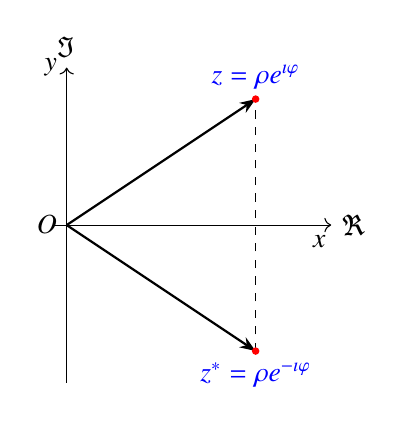
\begin{tikzpicture}[scale=0.8]
    \path (0,0) coordinate (origin);
    \path (4, 0) coordinate (x) ;
    \path (0, 2.5) coordinate (y) ;
    \path (3, 2.0) coordinate (z);
    \path (3,-2.0) coordinate (zminus);
    % \path (2.5, 2) coordinate (rho);
  
    \draw[->] (-0.2,0) --(4.2,0) node[right] {$\Re$};
    \draw[->] (0,-2.5) --(0,2.5) node[above] {$\Im$};
    \draw[solid, text=blue, thick, -{Stealth[length=2mm]}] (origin) -- (z) node[above] {$z=\rho e^{\imath \varphi}$};
    \draw[solid, text=blue, thick, -{Stealth[length=2mm]}] (origin) -- (zminus) node[below] {$z^{*}=\rho e^{-\imath \varphi}$};
    \draw[text=red, dashed]  (zminus) --(z) node[above]  {};
    % \draw[text=red, dashed] (y) --(z) node[above] {};
  
    \node at (origin) [left] {$O$};
    \node at (x) [below ]{$x$};
    \node at (y) [left ]{ $y$};
    % \node at (rho) [right] {$\rho$};
    \draw[color=red, fill=red] (z) circle (0.05);
    \draw[color=red, fill=red] (zminus) circle (0.05);
    % \draw pic["$\varphi$",draw, ->, angle eccentricity=1.2, angle radius=0.8cm]{angle = x--origin--z};
    % \draw pic["$\varphi$",draw, <-, angle eccentricity=1.2, angle radius=0.8cm]{angle = zminus--origin--x};

  \end{tikzpicture}
%   \caption{共轭的几何表示.} \label{fig:zminus}
% \end{figure} 
% \end{minipage}
\quad 
% \begin{minipage}{0.5\textwidth}
    % \begin{figure}[htb]
        % \centering
        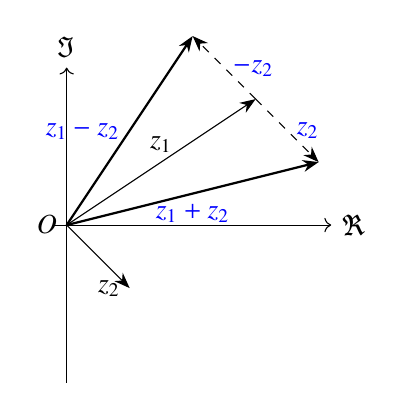
\begin{tikzpicture}[scale=0.8]
    % Define the vectors
    \path (3, 2.0) coordinate (z1);
    \path (1, -1.0) coordinate (z2);
    \path (4, 1) coordinate (z1pz2);
    \path (2, 3) coordinate (z1mz2);

    \draw[-{Stealth[length=2mm]}] (0,0) -- (z1) node[midway, above]{$z_1$};
    \draw[-{Stealth[length=2mm]}] (0,0) -- (z2) node[left]{$z_2$};
    % Draw the vector addition
    \draw[-{Stealth[length=2mm]}, text=blue, thick] (0,0) -- (z1pz2) node[midway, below]{$z_1 + z_2$};
    \draw[-{Stealth[length=2mm]}, text=blue, dashed] (z1) -- (z1pz2) node[midway, right]{$z_2$};

    % Draw the vector subtraction
    \draw[-{Stealth[length=2mm]}, text=blue, thick] (0,0) -- (z1mz2) node[midway, left]{$z_1 - z_2$};
    \draw[-{Stealth[length=2mm]}, text=blue, dashed] (z1) -- (z1mz2) node[midway, right]{$- z_2$};
    \path (0,0) coordinate (origin);
  
    \draw[->] (-0.2,0) --(4.2,0) node[right] {$\Re$};
    \draw[->] (0,-2.5) --(0,2.5) node[above] {$\Im$};
    \node at (origin) [left] {$O$};

  \end{tikzpicture}
    %   \caption{共轭的几何表示.} \label{fig:zminus}
    % \end{figure} 
% \end{minipage}
        \caption{左图:共轭$z^{*}$与$z$的关系; 右图:$z_1, z_2$的加减关系。}
\end{figure}
 

\begin{example}
讨论$\Re \frac{1}{z} = 2$在复平面上的意义。
\end{example}
\begin{solution}
    \begin{align*}
        \Re \frac{1}{z} &= 2\\
        \Re \frac{1}{x+\imath y} &  = 2 \\
        \frac{x}{x^2 +y^2} & = 2 。
    \end{align*}
因此,我们得到方程
\[
    (x-\frac{1}{4})^2 + y^2 = \left( \frac{1}{4}\right)^2,
\]
它表示以$(\frac{1}{4},0)$为圆心,$\frac{1}{4}$为半径的圆上各点集合。
\end{solution}
        

\begin{note}
    挑战自我: 试证明点 $a_1, a_2, a_3$ 当且仅当 
    $a_1^2+a_2^2+a_3^2=a_1 a_2+a_2 a_3+a_3 a_1$ 时为等边三角形的三个顶点。    
\end{note}
% \subsection{复数运算的几何表示}




% \subsubsection{}
\subsection{复变函数}
\label{sub:complexfunctions}

\subsubsection{定义}
\label{subsub:cmplx_func_def}

存在复数平面的点集$Z$,每一点$z\in Z$有一个或多个复数值$w$与之对应,则称$w$为$z$的函数--复变函数。$z$称为$w$的宗量,定义域为$Z$,记作
\begin{equation}
    w = w(z)\textrm{,} z\in Z \textrm{。}
\end{equation}
任意一个复变函数$w(z)$,$z=x + \imath y$,我们可以写称实部和虚部的组合,
\begin{align}
    w(z) = u(x,y) +\imath \; v(x,y) \textrm{,}
\end{align}
其中$u(x,y), v(x,y)$为纯实函数。它们可以类似的写成
\begin{align}
    \Re w(z) = u(x,y)\textrm{,} \quad \Im w(z) = v(x,y) \textrm{,}
\end{align}
$w(z)$的复共轭为$u(x,y) - \imath \; v(x,y)$。取决于$w(z)$,二者可能相等也可能不等。

这里我们列举一些常见复变函数。
\begin{itemize}
    \item 多项式:
        \begin{equation}
            a_0 + a_1 z + a_2 z^2 + \cdots + a_n z^n \textrm{,} \quad n\in \mathbb{Z}^+ \textrm{,}
        \end{equation}
    \item 有理分式:       
         \begin{equation}
        \frac{a_0 + a_1 z + a_2 z^2 + \cdots + a_n z^n}{{b_0 + b_1 z + b_2 z^2 + \cdots + b_m z^m}} \textrm{,} \quad  n,m\in \mathbb{Z}^+ \textrm{,}
        \end{equation}
    \item 根式:
        \begin{equation}
            (z-a)^{m/n} \textrm{,} \quad  n,m\in \mathbb{Z}^+ \textrm{,}
        \end{equation}
    \item 对数、指数
        \begin{equation}
            \ln z = \ln |z| + \imath \Arg z, \quad z^s = e^{s\ln z} \textrm{,}
        \end{equation}
    \item 正余弦,正余切函数 
        \begin{equation}
            \sin z , \cos z , \tan z, \cot z \textrm{,}
        \end{equation}
    \item 双曲正余弦, 双曲正余切函数
        \begin{equation}
            \sinh z , \cosh z , \tanh z, \coth z  \textrm{。}
        \end{equation}
\end{itemize}
以上所有出现的常数均为复数。

\begin{examplebox}{验证\begin{equation*}
    |\sin z|=\frac{1}{2} \sqrt{\left(e^{2 y}+e^{-2 y}\right)+2\left(\sin ^2 x-\cos ^2 x\right)} .
    \end{equation*}
    }
    由正弦函数定义得
    \begin{align*}
        \sin z &= \frac{e^{\imath z} - e^{-\imath z}}{2\imath} 
        \\ 
        & = \frac{e^{\imath x - y} - e^{-\imath x + y}}{2\imath}
        \\
        & = \frac{1}{2\imath}\left( e^{-y} (\cos x + \imath \sin x ) - e^{y} (\cos x - \imath \sin x ) \right) 
        \\
        & = \frac{1}{2\imath} \left( \cos x (e^{-y} - e^{y}) + \imath \sin x (e^{-y} + e^{y}) \right)
    \end{align*}
    取模后可得,
    \begin{align*}
        |\sin z | &= \frac{1}{2}\sqrt{ \cos^2x (e^{2y} + e^{-2y} -2) + \sin^2 x (e^{2y} + e^{-2y} +2) }
        \\
        &=\frac{1}{2}\sqrt{\left(e^{2 y}+e^{-2 y}\right)+2\left(\sin ^2 x-\cos ^2 x\right)}
    \end{align*}
    可见,与实函数不同的是,$|\sin z|$的取值完全可以大于$1$。
\end{examplebox}

复数
\begin{figure}
    \centering

    \input{tikz/branch_cut.tex}

\end{figure}
\section{解析函数}
% 
% \subsubsection{}
\subsection{复变函数}
\label{sub:complexfunctions}

\subsubsection{定义}
\label{subsub:cmplx_func_def}

存在复数平面的点集$Z$,每一点$z\in Z$有一个或多个复数值$w$与之对应,则称$w$为$z$的函数--复变函数。$z$称为$w$的宗量,定义域为$Z$,记作
\begin{equation}
    w = w(z)\textrm{,} z\in Z \textrm{。}
\end{equation}
任意一个复变函数$w(z)$,$z=x + \imath y$,我们可以写称实部和虚部的组合,
\begin{align}
    w(z) = u(x,y) +\imath \; v(x,y) \textrm{,}
\end{align}
其中$u(x,y), v(x,y)$为纯实函数。它们可以类似的写成
\begin{align}
    \Re w(z) = u(x,y)\textrm{,} \quad \Im w(z) = v(x,y) \textrm{,}
\end{align}
$w(z)$的复共轭为$u(x,y) - \imath \; v(x,y)$。取决于$w(z)$,二者可能相等也可能不等。

这里我们列举一些常见复变函数。
\begin{itemize}
    \item 多项式:
        \begin{equation}
            a_0 + a_1 z + a_2 z^2 + \cdots + a_n z^n \textrm{,} \quad n\in \mathbb{Z}^+ \textrm{,}
        \end{equation}
    \item 有理分式:       
         \begin{equation}
        \frac{a_0 + a_1 z + a_2 z^2 + \cdots + a_n z^n}{{b_0 + b_1 z + b_2 z^2 + \cdots + b_m z^m}} \textrm{,} \quad  n,m\in \mathbb{Z}^+ \textrm{,}
        \end{equation}
    \item 根式:
        \begin{equation}
            (z-a)^{m/n} \textrm{,} \quad  n,m\in \mathbb{Z}^+ \textrm{,}
        \end{equation}
    \item 对数、指数
        \begin{equation}
            \ln z = \ln |z| + \imath \Arg z, \quad z^s = e^{s\ln z} \textrm{,}
        \end{equation}
    \item 正余弦,正余切函数 
        \begin{equation}
            \sin z , \cos z , \tan z, \cot z \textrm{,}
        \end{equation}
    \item 双曲正余弦, 双曲正余切函数
        \begin{equation}
            \sinh z , \cosh z , \tanh z, \coth z  \textrm{。}
        \end{equation}
\end{itemize}
以上所有出现的常数均为复数。

\begin{examplebox}{验证\begin{equation*}
    |\sin z|=\frac{1}{2} \sqrt{\left(e^{2 y}+e^{-2 y}\right)+2\left(\sin ^2 x-\cos ^2 x\right)} .
    \end{equation*}
    }
    由正弦函数定义得
    \begin{align*}
        \sin z &= \frac{e^{\imath z} - e^{-\imath z}}{2\imath} 
        \\ 
        & = \frac{e^{\imath x - y} - e^{-\imath x + y}}{2\imath}
        \\
        & = \frac{1}{2\imath}\left( e^{-y} (\cos x + \imath \sin x ) - e^{y} (\cos x - \imath \sin x ) \right) 
        \\
        & = \frac{1}{2\imath} \left( \cos x (e^{-y} - e^{y}) + \imath \sin x (e^{-y} + e^{y}) \right)
    \end{align*}
    取模后可得,
    \begin{align*}
        |\sin z | &= \frac{1}{2}\sqrt{ \cos^2x (e^{2y} + e^{-2y} -2) + \sin^2 x (e^{2y} + e^{-2y} +2) }
        \\
        &=\frac{1}{2}\sqrt{\left(e^{2 y}+e^{-2 y}\right)+2\left(\sin ^2 x-\cos ^2 x\right)}
    \end{align*}
    可见,与实函数不同的是,$|\sin z|$的取值完全可以大于$1$。
\end{examplebox}

复数
\begin{figure}
    \centering

    \input{tikz/branch_cut.tex}

\end{figure}
\section{解析函数}

% \chapter{Introduction}
\label{ch:intro}


\section{Many-body problem}
% \chapter{Second Quantization}
\label{ch:2ndquan}


\section{Quantum Mechanics Review}
\label{sec:qmreview}
% \chapter{Green's Function}
\label{ch:gf}


\section{Green's Function}
% \part{复变函数论}

\subimport{complex/}{complex.tex}
\subimport{integral/}{integral.tex}
\subimport{calculus_variation/}{calculus_variation.tex}
\subimport{fourier/}{fourier.tex}
\subimport{laplace/}{laplace.tex}
\subimport{special/}{special.tex}
\subimport{mathphyequations/}{mathphyequations.tex}
\subimport{diffeq/}{diffeq.tex}
\subimport{separation/}{separation.tex}

% \part{数学物理方程}

% \subimport{chap07/}{chap07.tex}
% \subimport{chap08/}{chap08.tex}
% \subimport{chap09/}{chap09.tex}
% \subimport{chap10/}{chap10.tex}
% \subimport{chap11/}{chap11.tex}

\subimport{appendix/}{appendix.tex}
\end{document}